\documentclass[ALICE,manyauthors]{cernphprep}

\usepackage[comma,square,numbers,sort&compress]{natbib}
\usepackage{hyperref}
\usepackage{lineno}
%\usepackage{subcaption}
\usepackage{subfigure}
\usepackage[section]{placeins}
\usepackage {multicol}% Multi column in the table
\usepackage {multirow}% Multi row in the table
\usepackage {units}
\usepackage {array}
\linenumbers

% $Id: commands.tex 934 2013-06-19 20:56:45Z mfloris $

\newcommand{\mrm}[1]{\mathrm{#1}}
\newcommand{\mrmo}[1]{\mathrm{\overline{#1}}}
\newcommand{\bsb}[1]{\boldsymbol{#1}}
\newcommand{\circit}{\item[$\circ$]}

\newcommand{\ITS}          {\rm{ITS}}
\newcommand{\TOF}          {\rm{TOF}}
\newcommand{\ZDC}          {\rm{ZDC}}
\newcommand{\ZDCs}         {\rm{ZDCs}}
\newcommand{\ZNA}          {\rm{ZNA}}
\newcommand{\ZNC}          {\rm{ZNC}}
\newcommand{\SPD}          {\rm{SPD}}
\newcommand{\SDD}          {\rm{SDD}}
\newcommand{\SSD}          {\rm{SSD}}
\newcommand{\TPC}          {\rm{TPC}}
\newcommand{\VZERO}        {\rm{VZERO}}
\newcommand{\VZEROA}       {\rm{VZERO-A}}
\newcommand{\VZEROC}       {\rm{VZERO-C}}
\newcommand{\pip}          {$\pi^{+}$}
\newcommand{\pim}          {$\pi^{-}$}
\newcommand{\kap}          {K$^{+}$}
\newcommand{\kam}          {K$^{-}$}
\newcommand{\pbar}         {$\rm\overline{p}$}
\newcommand{\kzero}        {\ensuremath{{\rm K}^{0}_{S}}}
\newcommand{\kstar}        {\ensuremath{{\rm K}^{*}}}
\newcommand{\He}           {\ensuremath{^{3}{\rm He}}}
\newcommand{\LH}           {\ensuremath{^{3}_{\Lambda}{\rm H}}}
\newcommand{\vzero}        {\ensuremath{{\rm V}^0}}
\newcommand{\lmb}          {\ensuremath{\Lambda}}
\newcommand{\almb}         {\ensuremath{\bar{\Lambda}}}
\newcommand{\allpart}      {$\pi^{\pm}$, K$^{\pm}$, \kzero, p(\pbar) and \lmb(\almb)}
\newcommand{\allpi}        {$\pi^{\pm}$}
\newcommand{\allk}         {K$^{\pm}$}
\newcommand{\allp}         {p(\pbar)}
\newcommand{\alllmb}       {\lmb(\almb)}
\newcommand{\degree}       {$^{\rm o}$}
\newcommand{\dg}           {\mbox{$^\circ$}}
\newcommand{\dedx}         {\ensuremath{\mathrm{d}E/\mathrm{d}x}}
\newcommand{\dndy}         {d$N$/d$y$}
\newcommand {\ee}            {\mbox{e$^+$e$^-$}}
\newcommand{\pp}           {pp}
\newcommand{\ppbar}        {\mbox{$\mathrm {p\overline{p}}$}}
\newcommand{\PbPb}         {\mbox{Pb--Pb}}
\newcommand{\pPb}          {\mbox{p--Pb}}
\newcommand{\AuAu}         {\mbox{Au--Au}}
\newcommand{\pseudorap}    {\mbox{$\left | \eta \right | $}}
\newcommand{\dNdeta}       {\ensuremath{\mathrm{d}N_\mathrm{ch}/\mathrm{d}\eta}}
\newcommand{\dNdy}         {\ensuremath{\mathrm{d}N/\mathrm{d}y}}
\newcommand{\dNdptdy}      {\ensuremath{\mathrm{d}N/{\rm d}\pt\mathrm{d}y}}
\newcommand{\dNdyst}       {\ensuremath{\sqrt{\frac{dN_\pi/dy}{s_T}}}}
\newcommand{\dNdetatr}     {\mathrm{d}N_\mathrm{tracklets}/\mathrm{d}\eta}
\newcommand{\dNdetar}[1]   {\mathrm{d}N_\mathrm{ch}/\mathrm{d}\eta\left.\right|_{|\eta|<#1}}
\newcommand{\lum}          {\, \mbox{${\rm cm}^{-2} {\rm s}^{-1}$}}
\newcommand{\barn}         {\, \mbox{${\rm barn}$}}
\newcommand{\m}            {\, \mbox{${\rm m}$}}
\newcommand{\ncls}         {\ensuremath{N_{cls}}}
\newcommand{\nsigma}       {\ensuremath{n\sigma}}
\newcommand{\dcaxy}        {\ensuremath{{\rm DCA}_{xy}}}
\newcommand{\dcaz}         {\ensuremath{{\rm DCA}_{z}}}
\newcommand{\EcrossB}      {E$\times$B}%{\ensuremath{{\rm E}\times{\rm B}}}
\newcommand{\bb}           {Bethe-Bloch}
\newcommand{\s}            {\ensuremath{\sqrt{s}}}
\newcommand{\pt}           {\ensuremath{p_\mathrm{T}}}
\newcommand{\pT}           {\ensuremath{p_{\rm T}}}
\newcommand{\hlab}         {\ensuremath{\eta_{\rm lab}}}
\newcommand{\ynn}         {\ensuremath{y_{\rm NN}}}
\newcommand{\ycms}         {\ensuremath{y_{\rm CMS}}}
\newcommand{\ylab}         {\ensuremath{y_{\rm lab}}}
\newcommand{\ppi}          {\ensuremath{{\rm p}/\pi}}
\newcommand{\kpi}          {\ensuremath{{\rm K}/\pi}}
\newcommand{\lpi}          {\ensuremath{{\rm \Lambda}/\pi}}
%\newcommand{\ppi}          {\ensuremath{(\pi^+ + \pi^-)/({\rm K}^+ + {\rm K}^-)}}
%\newcommand{\kpi}          {\ensuremath{({\rm p} + {\rm \bar p})/({\rm K}^+ + {\rm K}^-)}}
\newcommand{\mt}           {\ensuremath{m_{\rm T}}}
\newcommand{\snn}          {\ensuremath{\sqrt{s_{\rm NN}}}}
\newcommand{\snnbf}        {\ensuremath{\mathbf{{\sqrt{s_{\mathbf NN}}}}}}
\newcommand{\sonly}        {\ensuremath{\sqrt{s}}}
\newcommand{\Npart}        {\ensuremath{N_\mathrm{part}}}
\newcommand{\avNpart}      {\ensuremath{\langle N_\mathrm{part} \rangle}}
\newcommand{\avNpartdata}  {\ensuremath{\langle N_\mathrm{part}^{\rm data} \rangle}}
\newcommand{\Ncoll}        {\ensuremath{N_\mathrm{coll}}}
\newcommand{\Dnpart}       {\ensuremath{D\left(\Npart\right)}}
\newcommand{\DnpartExp}    {\ensuremath{D_{\rm exp}\left(\Npart\right)}}
\newcommand{\dNdetapt}     {\ensuremath{\dNdeta\,/\left(0.5\Npart\right)}}
\newcommand{\dNdetaptr}[1] {\ensuremath{\dNdetar{#1}\,/\left(0.5\Npart\right)}}
\newcommand{\dNdetape}     {\left(\ensuremath{\dNdeta\right)/\left(\avNpart/2\right)}}
\newcommand{\dNdetaper}[1] {\ensuremath{\dNdetar{#1}\,/\left(\avNpart/2\right)}}
\newcommand{\dndydpt}      {\ensuremath{{\rm d}^2N/({\rm d}y {\rm d}p_{\rm t})}}
\newcommand{\abs}[1]       {\ensuremath{\left|#1\right|}}
\newcommand{\signn}        {\ensuremath{\sigma^{\rm inel.}_{\rm NN}}}
\newcommand{\vz}           {\ensuremath{V_{z}}}
\newcommand{\Tfo}          {\ensuremath{{T}_{\rm kin}}}
\newcommand{\Tch}          {\ensuremath{{T}_{\rm ch}}}
\newcommand{\bT}           {\ensuremath{\beta_{\rm T}}}
\newcommand{\avbT}         {\ensuremath{\left< \beta_{\rm T}\right>}}
\newcommand{\avpT}         {\ensuremath{\left< \pt \right>}}
\newcommand{\muB}          {\ensuremath{\mu_{B}}}
\newcommand{\stat}         {({\it stat.})}
\newcommand{\syst}         {({\it sys.})}
\newcommand{\Fig}[1]       {Fig.~\ref{#1}}
\newcommand{\Figure}[1]    {Figure~\ref{#1}}
%\newcommand{\Ref}[1]       {Ref.~\cite{#1}}
%\newcommand{\green}[1]     {\textcolor{green}{#1}}
%\newcommand{\blue}[1]      {\textcolor{blue}{#1}}
%\newcommand{\red}[1]       {\textcolor{red}{#1}}
%\newcommand{\white}[1]     {\textcolor{white}{#1}}
\newcommand{\gevc}         {\ensuremath{{\rm GeV}/c}}
\newcommand{\mevc}         {\ensuremath{{\rm MeV}/c}}
\newcommand{\gs}           {\ensuremath{\gamma_{s}}}
\newcommand{\gq}           {\ensuremath{\gamma_{q}}}
\newcommand{\gc}           {\ensuremath{\gamma_{c}}}
\newcommand{\chindf}       {\ensuremath{\chi^{2}/{\rm NDF}}}
\newcommand{\avg}[1]       {\ensuremath{\left\langle#1\right\rangle}}
\newcommand{\etalab}       {\ensuremath{\eta_{{\rm lab}}}}
\newcommand {\gammas}			{\ensuremath{\gamma_{\mathrm{s}}}}

\newcommand{\DNDETAINEL}{5.31~$\pm$~0.18\xspace}
\newcommand{\DNDETAINELGTZERO}{6.46~$\pm$~0.19\xspace}
\newcommand{\DNDETAINELGTZEROONE}{6.61~$\pm$~0.20\xspace}

\newcommand{\inelgtzero}{INEL$>$0\xspace}
\newcommand{\average}[1]{\ensuremath{\langle #1 \rangle}\xspace}
\newcommand{\mpt}        {\ensuremath{\langle\pt\rangle}\xspace}
\newcommand{\nch}        {\ensuremath{N_\mathrm{ch}}\xspace}
\newcommand{\mnch}      {\ensuremath{\langle\nch\rangle}\xspace}
\newcommand{\nchacc}        {\ensuremath{N_\mathrm{ch}^\mathrm{acc}}\xspace}
\newcommand{\mnchacc}      {\ensuremath{\langle\nchacc\rangle}\xspace}
\newcommand{\inelg}     {\ensuremath{\mathrm{INEL}_{>0}}}



\newcommand{\dndeta}{\ensuremath{{\rm d}N_{\rm ch}/{\rm d}\eta}\xspace}
\newcommand{\dndpt}{\ensuremath{{\rm d}N_{\rm ch}/{\rm d}\pt}\xspace}
\newcommand{\etaless}[1]{\ensuremath{\left|\eta\right| < #1}\xspace}
\newcommand{\dndetaless}[1]{\ensuremath{{\rm d}N_{\rm ch}/{\rm d}\eta|_{\etaless{#1}}}\xspace}
\newcommand{\avdndeta}{\ensuremath{\langle \dndeta \rangle}}
\newcommand{\zvtx}{\ensuremath{z_\mathrm{vtx}}}
\newcommand{\pythiae}{\ensuremath{\mathrm{PYTHIA}\,8}}
%\newcommand{\pythiam}{\ensuremath{\mathrm{PYTHIA}\,8\,\mathrm{Monash}\,2013}}
\newcommand{\pythiam}{\ensuremath{\mathrm{PYTHIA}\,8\,\mathrm{tune}}{\text -}4c}
\newcommand{\pythiashoving}{{\ensuremath{\mathrm{PYTHIA}\,8~\mathrm{String}~}}\ensuremath{\mathrm{Shoving}}}
\newcommand{\epos}{{\ensuremath{\mathrm{EPOS}\,~\mathrm{LHC}}}}
%\newcommand{\pythiashoving}{\ensuremath{\mathrm{PYTHIA}\,8~\mathrm{String}~}\linenomath{-}\ensuremath{\mathrm{Shoving}}}
\newcommand{\pttrig}{\ensuremath{p_\mathrm{T,\,trig}}}
\newcommand{\ptassoc}{\ensuremath{p_\mathrm{T,\,assoc}}}
\newcommand{\ptjet}{\ensuremath{p_\mathrm{T,\,Jet}}}
\newcommand{\ptlead}{\ensuremath{p_\mathrm{T,\,LP}}}
\newcommand{\pttrigassoc}{\ensuremath{p_\mathrm{T,\,trig\,(assoc)}}}









\renewcommand{\labelitemi} {$-$}
%==========================================================%
%%% inline warnings for internal discussion
%\newcommand{\warn}[1]      {\textbf{\textcolor{red}{[#1]}}}
\newcommand{\warn}[1]      {{\small\textbf{\textcolor{red}{(!\footnote{\textbf{(!)}~#1})}}}}
\newcommand{\warnin}[1]         {\textit{\textcolor{red}{(#1)}}}
%\newcommand{\warn}[1]      {#1}
%\newcommand{\warn}[1]      {{\small\textbf{(!\footnote{\textbf{(!)}~#1})}}\marginpar{\textbf{---}}}
\newcommand{\todo}[1]      {\textbf{\textcolor{red}{[TODO: #1]}}}
%%% fake numbers
\newcommand{\fake}[1]      {\textbf{\textcolor{red}{#1}}}
%\newcommand{\fake}[1]      {#1}
\newcommand{\final}[1]     {\textbf{\textcolor{blue}{#1}}}
\newcommand{\prelim}[1]    {\textbf{\textcolor{magenta}{#1}}}
\renewcommand{\mod}[1]       {\textbf{\textcolor{red}{#1}}}

\begin{document}

%%%%%%%%%%%%%%%  Title page %%%%%%%%%%%%%%%%%%%%%%%%
\begin{titlepage}

\PHyear{}
\PHnumber{2019-xxx}      % required, will be obtained from PH
%\PHdate{Day Month}  % required, will be obtained from PH
\PHdate{\today}
%

%%% Put your own title + short title here:
\title{Long range correlations and their event scale dependence in high multiplicity pp collisions at $\sqrt{s}$ =13 TeV}
\ShortTitle{Long-range correlations in pp collisions}   % appears on right page headers

%%% Do not change the next lines
%\Collaboration{ALICE Collaboration\thanks{See Appendix~\ref{app:collab} for the list of collaboration members}}
\ShortAuthor{ALICE Collaboration} % appears on left page headers, do not change

\begin{abstract}
%The observed azimuthal modulations of long-range correlations in pseudorapidity in small systems like pp or p-Pb collisions show strikingly similar features to those seen in heavy ion collisions. Many theoretical approaches to interpreting this effect have been developed. However, it is still unclear whether these long-range correlations are due to final or initial state effects. To further investigate these effects, we studied long-range correlations as a function of transverse momentum in very high multiplicity pp collisions at $\sqrt{s} =13$ TeV, collected with the high multiplicity event trigger during 2016 and 2017 with ALICE. In this talk, we present the near-side per-trigger yield at large pseudorapidity separation (ridge yield) as a function of transverse momentum in pp collisions at $\sqrt{s} =13$ TeV. The results are compared to previous measurements from CMS experiments. In addition, we present the ridge yield in events where harder fragmentation processes are present, to explore possible physical origins of long-range correlations.



In recent years, similar features between small systems like proton-proton (pp) collisions and large systems like lead-lead collisions have been observed via long-range correlations in pseudorapidity (so-called the ridge) for pairs of charged hadrons. Many theoretical approaches have been applied to interpret the similarity. However, it is still controversial whether the ridge in small systems is originated from initial or final-state effects of the collision. To further investigate these effects on the ridge effect, we present the new results of long-range correlations as a function of transverse momentum of jets in very high-multiplicity pp collisions at center-of-mass energy $\sqrt{s} = 13$~TeV. The study benefit from a dedicated high-multiplicity trigger implemented in ALICE since 2016 because of increased statistics for high-multiplicity pp collisions.  The results are compared to previous measurements by other LHC experiments. In addition, we explore possible physical origins of the ridge effects in small systems by studying the results as a function of the energy scale of the hard fragmentation process and comparing the various theoretical models tuned for the initial and final state effect.
\end{titlepage}
\setcounter{page}{2}

% !TEX root = paper.tex

\section{Introduction}
\label{sec:intro}

Strong collectivity observed in the azimuthal correlations of particles emitted over a wide pseudorapidity range, in high-energy nucleus-nucleus collisions at RHIC~\cite{Adams:2005dq,Adcox:2004mh,Arsene:2004fa,Back:2004je} and LHC~\cite{Abelev:2012di, Abelev:2014pua, ATLAS:2011ah}, indicates the formation of a strongly interacting matter called the quark-gluon plasma (QGP), which exhibits hydrodynamic behavior (see the reviews~\cite{Romatschke:2007mq,Jeon:2015dfa,Romatschke:2017ejr}). The recent efforts are focused on constraining the transport properties of the QGP in hydrodynamic models~\cite{Niemi:2015qia,Bernhard:2016tnd,Bernhard2019} along with few advanced experimental efforts~\cite{ALICE:2016kpq,Acharya:2017gsw,Acharya:2017zfg,Acharya:2020taj}.
In recent years similar collective behaviors via long-range azimuthal correlations are also observed for small systems with high final-state particle multiplicity such as proton-proton (pp)~\cite{Aad:2015gqa,Khachatryan:2015lva,Khachatryan:2016txc,Acharya:2019vdf}, proton-nucleus (pA)~\cite{Abelev:2012ola,Aad:2014lta,Aaboud:2016yar,Khachatryan:2016ibd}, and lighter nucleus-nucleus systems~\cite{PHENIX:2018lia,Aidala:2017ajz}, revealing strong indications for collective flow with hydrodynamic characteristics even in small systems, though the volume and lifetime of the medium produced by such a system are expected to be small. 

Measurements of two-particle angular correlations are typically performed in terms of two dimensional $\Delta\eta-\Delta\varphi$ correlation functions, where $\eta$ is the pseudorapidity and $\varphi$ is the azimuthal angle. Long-range structure of two-particle correlation functions is of particular interest in studies of possible novel collective effects, where the effects of known sources such as resonance decays and fragmentation of high-momentum partons are known to be small. For most Monte Carlo (MC) event generators in pp collisions, the typical sources of such long-range correlations are momentum conservation and away-side ($\Delta\varphi$ $\approx$ $\pi$ ) jet correlations.
The enhancement in the associated yield of two-particle correlations at small relative azimuthal angle ($\Delta\varphi$) that extends over a long-range of relative pseudorapidity ($\Delta\eta$), is dubbed ``ridge'' due to its shape in the $\Delta\eta-\Delta\varphi$ plane.
The shape of these $\Delta\varphi$ correlations can be studied via a Fourier decomposition~\cite{Poskanzer:1998yz,Voloshin:2008dg}. The second and third order terms are the dominant harmonic coefficients $v_n$. The $v_n$ coefficients can be related to the collision geometry and density fluctuations of the colliding nuclei~\cite{Alver:2010gr,Alver:2010dn,ALICE:2011ab} and to the transport properties of the QGP in relativistic viscous hydrodynamic models~\cite{Gale:2012rq,Niemi:2015qia,Shen:2014vra,Bernhard:2016tnd,Bernhard2019}.

% TODO more pA measurements
The ridge structures in high-multiplicity pp and p--Pb events have been attributed to mechanisms like initial-state effects, such as gluon saturation~\cite{Dusling:2012cg,Bzdak:2013zma} and color reconnections~\cite{Ortiz:2013yxa,Sarma:2019teo} forming along the longitudinal direction and final-state effects, such as parton-induced interactions~\cite{Arbuzov:2011yr}, and collective effects due to a hydrodynamic behavior of the produced particles arising in a high-density system possibly formed in these collisions~\cite{Weller:2017tsr,Zhao:2017rgg}. 
Hybrid models implementing both effects are generally used in hydrodynamic simulations~\cite{Greif:2017bnr,Mantysaari:2017cni}. 
The proton shape and its fluctuations are also important to model the small systems \cite{Mantysaari:2017cni}.
The hydrodynamics itself might not be the only mechanism of the observed collectivity~\cite{Zhao:2020pty}. 
The influence and interplay of initial state and final state effects are recently studied carefully for the first time in ~\cite{Greif:2019ygb}, pointing out that the details of the initial state are crucially important for the quantitative description of observables in small systems~\cite{Schenke:2019pmk}. 
The attempts to describe the collective effects systematically from the small to large systems are being made experimentally~\cite{Acharya:2019vdf} and theoritically~\cite{Greif:2019ygb}.
However, a quantitative description of the full set of experimental data has not been achieved yet.
The summary of various explanations for the observed correlations in these small systems are summarized in ~\cite{Strickland:2018exs,Loizides:2016tew,Nagle:2018nvi}.

Furthermore, if collectivity in small systems is due to final state interactions, it is expected to measure its effect on jets. Proving the presence of jet quenching will be another crucial milestone to demonstrate the existence of the final-state effect in high-multiplicity pp collisions. The most of observables for the jet quenching in pp and p--Pb collisions do not show any clear evidences so far~\cite{Khachatryan:2016odn,Adam:2016jfp,Adam:2016dau,Acharya:2017okq}. The difficulties are attributed to an ambiguous reference since the hard probes themselves are also enhanced by requiring high multiplicity in the event~\cite{Adam:2016jfp,Acharya:2018egz}.

%Small system studies: A theory overview 1807.07191 Strickland:2018exs
%find one more one this regard.
The ATLAS experiment recently showed that the ridge remains in events tagged with a Z-boson~\cite{Aaboud:2019mcw}, possibly with an accompanying jet.
The impact parameter dependence on dijet or multi-jet production in pp collisions was studied in \cite{Frankfurt:2003td}.
The microscopic model for collectivity, based on interacting string implemented in the PYTHIA8 event generator so called the ``shoving model''~\cite{Bierlich:2017vhg} , can qualitatively reproduce the CMS near-side ridge yield~\cite{Khachatryan:2016txc}. This challenges the hydrodynamic picture and predicts modifications to jet fragmentation
properties~\cite{Bierlich:2019ixq}.

% check this paper https://arxiv.org/abs/1910.13978 ATLAS pt cut...
% Bierlich:2017vhg (Shoving) Bierlich:2019ixq  
% add vn extractio??
% flow vn extraction : awayside ??
% 
% AA geometry dominant for v2 and what about in pp, b vs v2 or ridge..
% Frankfurt:2003td
% Aaboud:2019mcw Z-tagged ridge ATLAS

To further investigate these effects, we studied long-range correlations as a function of transverse momentum in very high multiplicity pp collisions at $\sqrt{s} =13$ TeV, collected with the high multiplicity event trigger during the LHC Run 2 data taking period. In this article, we present the near-side per-trigger yield at large pseudorapidity separation as a function of transverse momentum. The results are compared to previous measurements from CMS experiments. In addition, we report the ridge yield in events where harder fragmentation processes are present, to explore possible physical origins of long-range correlations.


The experimental setup and analysis method are described in Sec.~\ref{sec:experiment} and \ref{sec:ana}, sequentially.  The sources of systematic uncertainties are represented in Sec.~\ref{sec:uncertainties}. The results of the measurements are interpreted in Sec.~\ref{sec:results}. In Sec.~\ref{sec:theory} we report comparisons to model calculations.
Finally, Sec.~\ref{sec:summary} summarizes our new results.

 %h has indicated the formation of a strongly interacting quark-gluon plasma (QGP) matteras indicated the formation of a strongly interacting quark-gluon plasma (QGP) matter
% !TEX root = paper.tex

\section{Experimental setup}
\label{sec:experiment}

%LHC at CERN produces various interesting phenomena including the ridge effect that is the main topic of the document in pp collisions with the highest center-of-mass energy in the world.
%Recent center-of-mass energy in pp collisions reaches up to $\sqrt{s} = 13$~TeV during the last LHC Run 2 period. 
The analysis is based on the data sets in pp collisions at $\sqrt{s} = 13$~TeV collected from 2016 to 2018 in the LHC Run 2 period.  The full description of ALICE detector in the LHC Run 2 can be found in Refs.~\cite{Aamodt:2008zz,Abelev:2014ffa}. The present analysis mainly utilizes V0~\cite{Abbas:2013taa}, ITS (Inner Tracking System)~\cite{aliceITS} and TPC (Time Projection Chamber)~\cite{aliceTPC} detectors.


The V0 detector consists of two rings, V0-A and V0-C, each made of 32 scintillator tiles, covering the full azimuthal angle within 2.8$<\eta<$5.1 and -3.7$<\eta<$-1.7, respectively. The V0 provides trigger and estimation of event multiplicity. A sample of events including higher numbers of produced particles is obtained with a high multiplicity trigger, which is achieved by requiring some thresholds on signal amplitudes of energy deposit by charged particles in the V0 detector.

Charged particles are reconstructed by the ITS and TPC, which are working in a constant solenoidal magnetic field of 0.5~T.  The ITS is composed of three sub-systems, Silicon Pixel Detector(SPD), Silicon Drift Detector (SDD) and Silicon Strip Detector (SSD). The ITS and TPC covering the full azimuthal region have acceptances up to $|\eta| < 1.4$ and 0.9, respectively, for detection of charged particles with a primary vertex in $|z_\mathrm{vtx}|<10$~cm. The tracking of charged particles is done with the combined information of the ITS and TPC that enables the reconstruction of tracks down to 0.2~GeV/$c$ with a $\sim $75\% efficiency.


%The multiplicity class is classified by the signal amplitude of the V0 detector.
The multiplicity class used in the present analysis is the top 0.1\% signal amplitude events by the V0 detector for the set of minimum bias events at ALICE. Corresponding number of charged particles is reported as $\sim$31 in the mid-rapidity region ($|\eta|<0.5$) that is almost 5 times larger than the minimum-bias events.  Statistics of the high multiplicity event benefits from a dedicated high multiplicity trigger that was recently implemented at ALICE  in the LHC Run 2 period.  
 


\section{Analysis Procedure}
\label{sec:ana}

The two-particle correlation between trigger particle and associated particle is measured as function of relative pseudo rapidity($\Delta\eta$) and azimuthal angle($\Delta\varphi$). The following equation expresses the correlation function as associated yield per trigger particle as function of $\Delta\eta$ and $\Delta\varphi$ with a given transverse momentum($\it{p}_{\rm{T, trig}}$, $\it{p}_{\rm{T, assoc}}$) of trigger particles and associated particles.
%with the notation of $\it{p}_{\rm{T, trig}} > \it{p}_{\rm{T, assoc}}$.
\begin{eqnarray}
\frac{1}{N_{\rm{trig}}} \frac{ \rm{d}\it{}^{2} N_{\rm{pair}} }{ \rm{d} \Delta\eta \rm{d}\Delta\varphi} = B(0, 0)\frac{S(\Delta\eta, \Delta\varphi)}{B(\Delta\eta, \Delta\varphi)},
\end{eqnarray}
where the $N_{\rm{trig}}$ is the number of trigger particles in the corresponding multiplicity class. The signal distribution $S(\Delta\eta, \Delta\varphi)$ is constructed using two-particle correlation in the same event and the background distribution $B(\Delta\eta, \Delta\varphi)$ is constructed using two-particle correlation in mixed events having the same primary vertex and belonging to the same multiplicity class considering the change of acceptance effect with respect to the multiplicity class and primary vertex.

The quantitative study of ridge is done with $\Delta\varphi$ distribution at large $\Delta\eta$ to achieve direct comparison of ridges between different event classes and transverse momentum intervals. The large $\Delta\eta$ range is defined as 1.6$<|\Delta\eta|<$1.8, which allows non-flow effects, mainly coming from the jet, not to contribute to the $\Delta\varphi$ distribution.
\begin{eqnarray}
\frac{1}{N_{\rm{trig}}} \frac{ \rm{d}\it{}N_{\rm{pair}} }{ \rm{d}\Delta\varphi } = \int_{|\Delta \eta|>1.6} \rm{d} \Delta \eta \frac{1}{\it{N}_{\rm{trig}}} \frac{ \rm{d}\it{}^{2} N_{\rm{pair}} }{ \rm{d}\Delta\eta \rm{d}\Delta\varphi}
\end{eqnarray}
The baseline of the correlations is subtracted by implementing Zero-Yield-At-Minimum (ZYAM) procedure. The minimum yield ($C_{\rm{ZYAM}}$) at the minimum $\Delta\varphi$($\Delta\varphi_{\rm{min}}$) of the $\Delta\varphi$ distribution are obtained from the function, which fits the $\Delta\varphi$ distribution with Fourier series up to the third harmonic. Subtracting $C_{\rm{ZYAM}}$ from the $\Delta\varphi$ distribution makes the yield at $\Delta\varphi_{\rm{min}}$ zero in order to describe the shape to find the minimum to be used for integral of the yield. The associated yield of the ridge($Y^{\rm{assoc}}$) is obtained by integrating the near-side peak of the $\Delta\varphi$ distribution over $|\Delta\varphi|<|\Delta\varphi_{\rm{min}}|$ after ZYAM.
\begin{eqnarray}
Y^{\rm{assoc}} = \int_{|\Delta \varphi| < |\Delta\varphi_{\rm{min}}| } \rm{d} \Delta\varphi \frac{1}{\it{N}_{\rm{trig}}} \frac{ \rm{d}\it{}N_{\rm{pair}} }{ \rm{d}\Delta\varphi } 
\end{eqnarray}

The ridge yield is further studied with various event selections regarding hard processes. The event selection is applied by requiring minimum transverse momentum of leading track or jet reconstructed in the mid-rapidity. The leading track is accepted within $|\Delta\eta|<0.9$ and reconstructed jet, which are made with anti-$k_{\rm{T}}$ algorithm with cone radius as 0.4, is accepted within $|\Delta\eta|<0.4$. The transverse momentum of jet is also corrected with underlying event density($\rho \cdot A$). The high $\it{p}_{\rm{T}}$ track and jet mostly generated from the hard scatterings in the initial collisions of hadrons so that tagging of events with transverse momentum of leading track or jet allows us to access to the high momentum transfer from the collisions to the initial partons.

Monte Carlo simulation with PYTHIA8 event generator and with particle transport through the detector using GEANT simulation has been used to estimate the charged single particle efficiency and the contamination from the non-primary particle. 

%The corrections have been tested by comparing the distributions, which are constructed with generated true particles and reconstructed particles with detector responses. The several percentage of non-closure has been considered into systematic uncertainty.

\section{Systematic Uncertainty}
\label{sec:uncertainties}
The systematic uncertainty is evaluated by varying the event selection, track selection, yield extraction procedures and efficiency correction. Each source is separated into individual parts. The uncertainty from the event selection can be divided into Pile-up rejection and primary vertex selection. The uncertainty from the track selection is estimated by changing the selection criteria. The uncertainty from the yield extraction procedures can be divided into long-range definition and ZYAM procedure. The uncertainty from the efficiency correction is estimated by enlarging the event mixing bins, which is relevant to acceptance correction. Finally, The uncertainty from the application of track efficiency correction is estimated comparing the results constructed by efficiency corrected tracks with the results constructed by true particles. The uncertainty of $Y^{\rm{assoc}}(\it{p}_{\rm{T, trig}},\,\it{p}_{\rm{T, assoc}})$ is summarized by averaging the each uncertainty for a given $\it{p}_{\rm{T, trig}},\,\it{p}_{\rm{T, assoc}}$. The uncertainty of $Y^{\rm{assoc}}(\it{p}_{\rm{T, Lead}})$ or $Y^{\rm{assoc}}(\it{p}_{\rm{T, Jet}})$ is summarized by averaging the each uncertainty for a given $\it{p}_{\rm{T, Lead}}$ or $\it{p}_{\rm{T, Jet}}$ selection.
\begin{table}[!h]
\caption{ The relative systematic uncertainty(\%) of the associated yield spectrum as function of $(\it{p}_{\rm{T, trig}},\,\it{p}_{\rm{T, assoc}})$(second), $\it{p}_{\rm{T,Lead}}$(thrid) or $\it{p}_{\rm{T,jet}}$(fourth) selection in high multiplicity(0-0.1\%) }
\centering
\begin{tabular}{|c|<{\centering}m{8em}|<{\centering}m{6em}|<{\centering}m{6em}|}
\hline 
Sources & Uncertainty $Y^{\rm{assoc}}(\it{p}_{\rm{T, trig}},\,\it{p}_{\rm{T, assoc}})$ & Uncertainty $Y^{\rm{assoc}}(\it{p}_{\rm{T, Lead}})$ & Uncertainty $Y^{\rm{assoc}}(\it{p}_{\rm{T, Jet}})$ \\ \hline \hline
Pileup cut			& $\sim$0.8	&0-4		&0-4		\\ \hline
Primary Vertex		& $\sim$2.4	&1-12	&1-8		\\ \hline

Tracking			& $\sim$4.0 	&2		&2		\\ \hline

ZYAM			& $\sim$5.1	&2		&2		\\ \hline
$\Delta\eta$ range	& $\sim$4.5	&3-7		&3-9		\\ \hline

Mixing			& $\sim$4.4	&2-8		&1-16	\\ \hline

M.C. non-closure*	& $\sim$2.5 	&1		&1		\\ \hline
Total 			& $\sim$9.7	&4-16	&4-22	\\ 
\hline 
\end{tabular}

\end{table}

The uncertainty from the pileup rejection is estimated by inspecting the changes of results with different rejection methodologies from the default one. The estimated uncertainty is 1\% without $\it{p}_{\rm{T, Lead}}$ or $\it{p}_{\rm{T, Jet}}$ selection. The uncertainty is increased up to 4\% with $\it{p}_{\rm{T, Lead}}$ or $\it{p}_{\rm{T, Jet}}$ selection.

The uncertainty from the primary vertex selection along the beam axis is estimated by varying the selection range of primary vertex from $|z_{vtx}|<$ 8 cm to $|z_{vtx}|<$ 6 cm. The narrower primary vertex selection allows one to accept more forward tracks, which could be very sensitive to select long-range side. The estimated uncertainty is increased up to 12\% from 1\%, which is obtained without the event scale selection.

The uncertainty from the track selection is estimated by varying the track selection methodologies from the one optimized for refining the angular track distribution to the other optimized for particle identification. The estimated uncertainty for track selection is 4\% by averaging the uncertainty for whole transverse momentum bins and 2\% for 1$<\it{p}_{\rm{T}}<$2 GeV/\it{c}\rm{} tracks.

The uncertainty from the ZYAM procedure is estimated by varying the finding-scope for minimum position. The estimated uncertainty for track selection is 5.1\% by averaging the uncertainty for whole transverse momentum bins and 2\% for 1$<\it{p}_{\rm{T}}<$2 GeV/\it{c}\rm{} tracks, which is not largely affected by the event scale selection.

The uncertainty from the long $\Delta\eta$ range is estimated by varying the $\Delta\eta$ range. The uncertainty might include effects from the longitudinal de-correlations and possible non-flow contamination, which is thought be small. The estimated uncertainty is increased up to 9\% from 3\%, which is obtained by averaging the whole transverse momentum range.

The uncertainty from the mixing pool bin size of primary vertex is estimated by varying the bin size from 2.0 cm to 1.0 cm. The estimated uncertainty is 1-16\%

*The M.C. closure test for efficiency correction results in $\sim$2.5\% discrepancy. The discrepancy is considered into systematic uncertainty.



\iffalse


\begin{table}[!h]
\centering
\caption{ Summary of the systematic uncertainties. See text for details.}
\begin{tabular}{ c|c }
%\begin{tabular}{c || c}
\hline
Source &  Uncertainty \\ \hline
Event mixing & 6-10\% \\  \hline
$\Delta\eta$ projection range & 10-15\% \\ \hline
M.C. closure & 4\% \\ \hline
Primary vertex & 4\% \\ \hline
Pileup Cut & 4\% \\ \hline
Track selection & 5\% \\ \hline
Total & 14-20\% \\
\hline
\end{tabular}
%\caption{ Definition of multiplicity class in this analysis. Reference definition of multiplicity coud be found in the following link; \url{https://twiki.cern.ch/twiki/bin/viewauth/ALICE/ReferenceMult}  }
\end{table}
\fi





% !TEX root = paper.tex

\section {Results}
\label{sec:results}

The two-dimensional associated yield per trigger particle is shown in Figure 1 for pairs of trigger particle and associated particle with 1.0$<\it{p}_{\rm{T, assoc}}<\it{p}_{\rm{T, trig}}<$2.0 GeV/\it{c}\rm{} in pp collisions at $\sqrt{\it{s}} = $\unit{13} {\rm{}TeV} in the 0-0.1\% (left), 5-20\% (middle) and 20-100\% (right) multiplicity class estimated by V0 detector, which covers forward rapidity region. The ridge is clearly seen in high multiplicity class unlike in lower multiplicity classes.


\begin{figure}
	\centering
	\subfigure{ 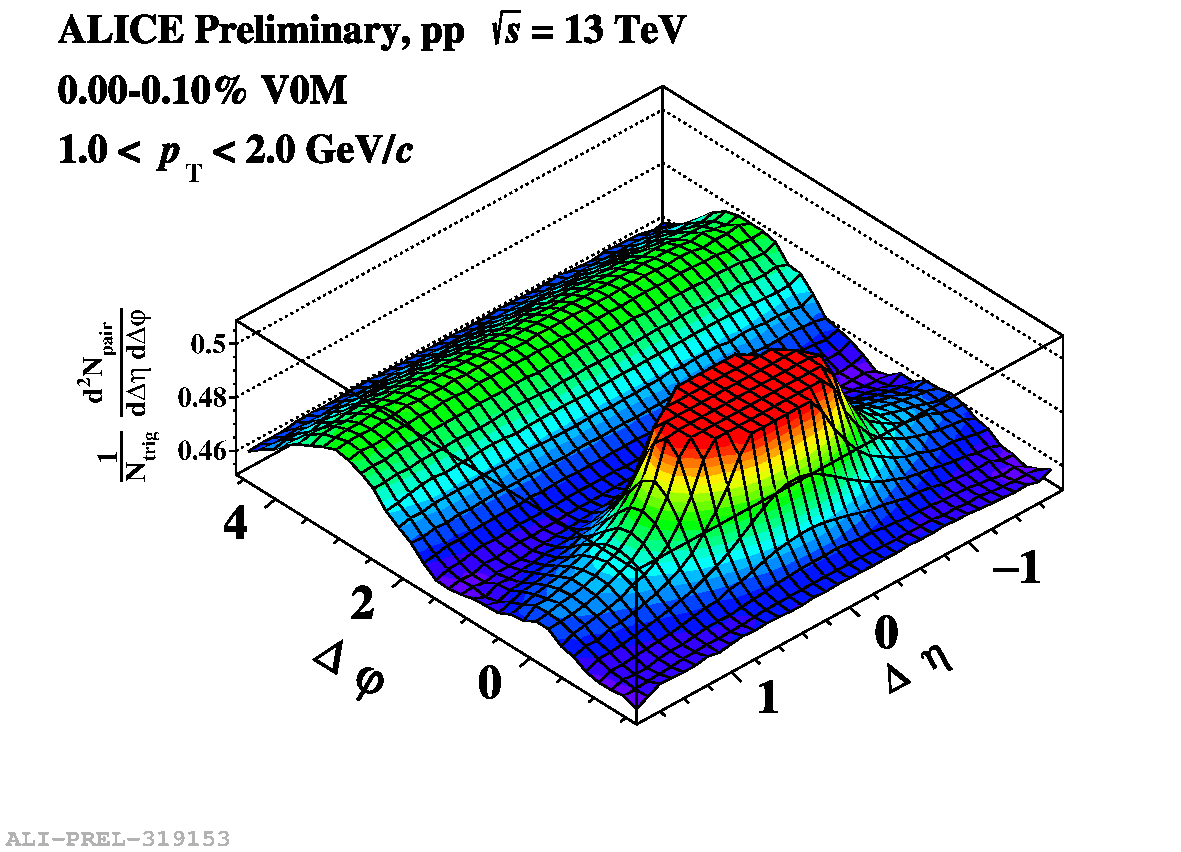
\includegraphics[width=0.31\textwidth]{./figures/corr1.pdf} }
	\subfigure{ 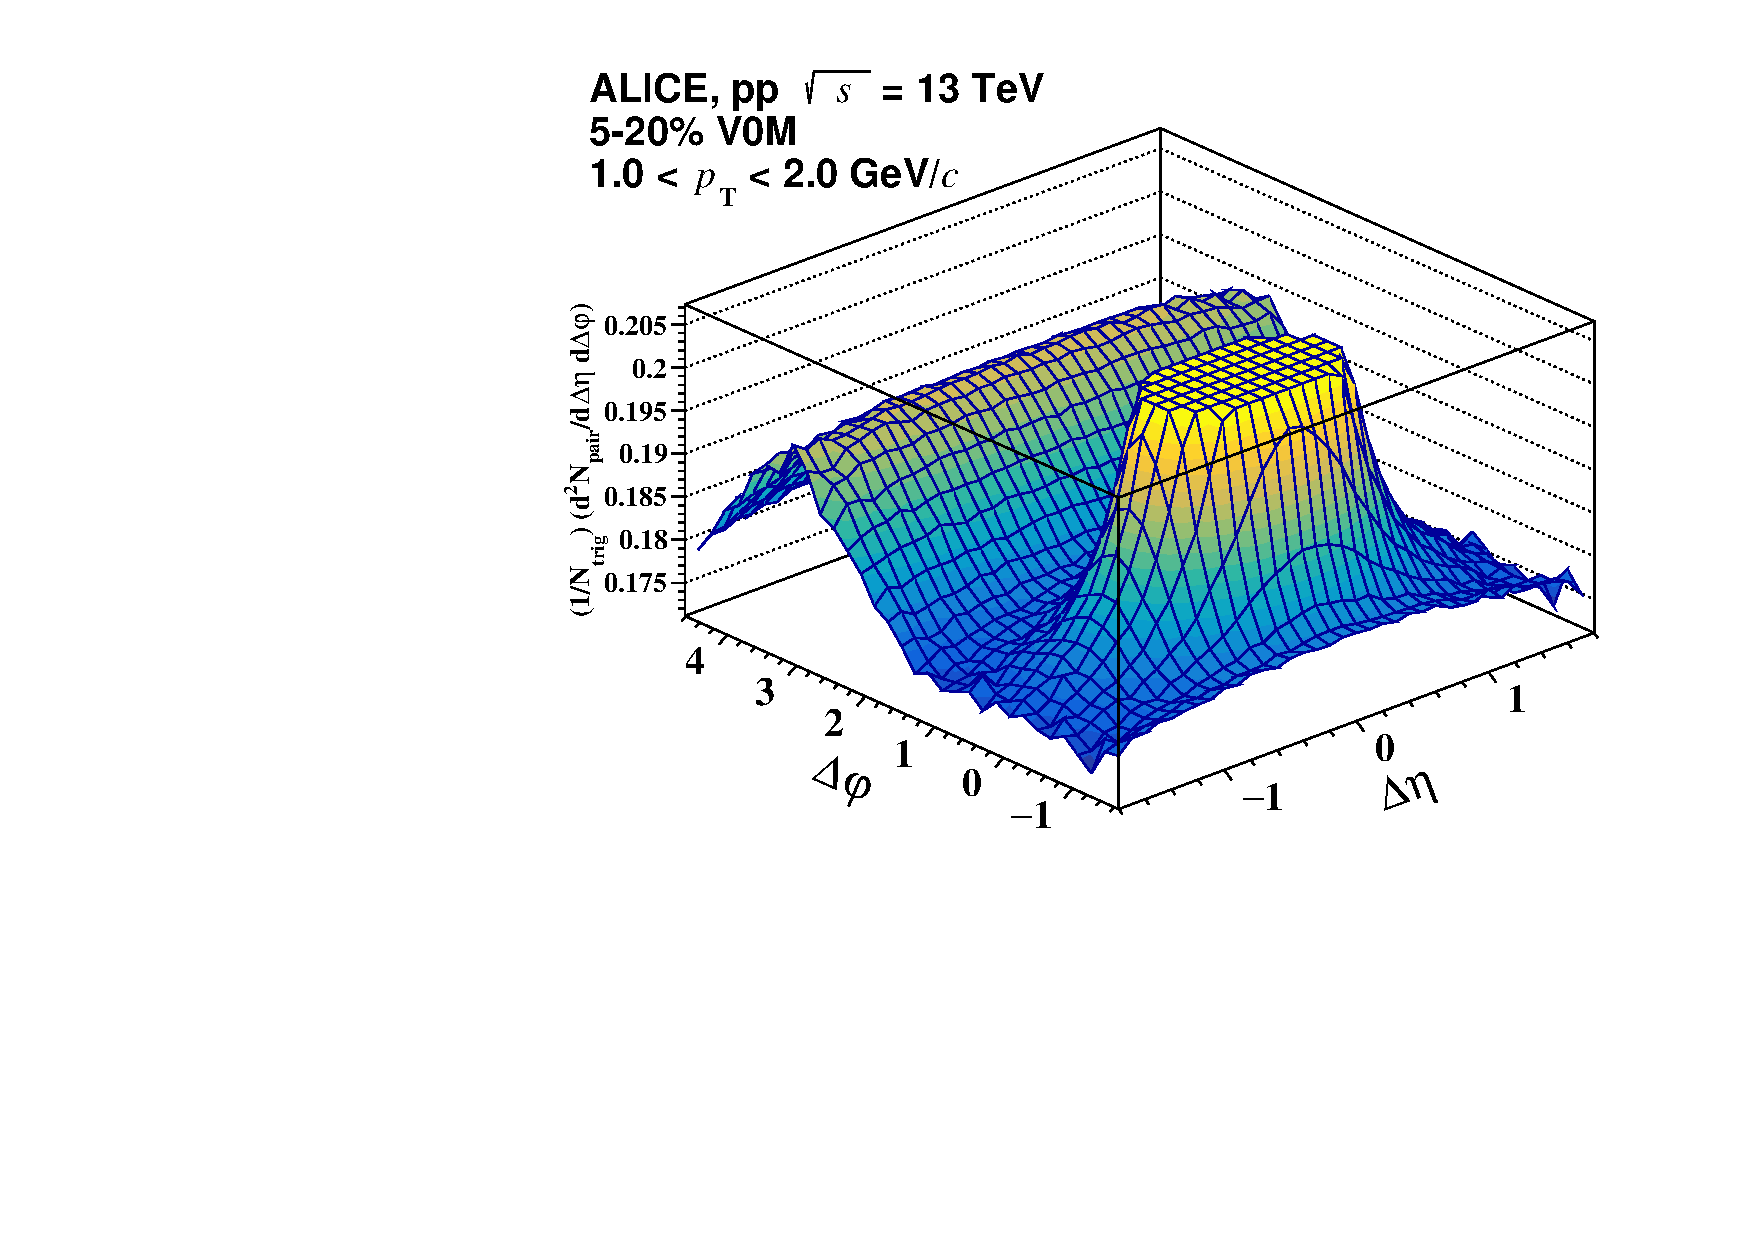
\includegraphics[width=0.31\textwidth]{./figures/corr2.pdf} }
	\subfigure{ 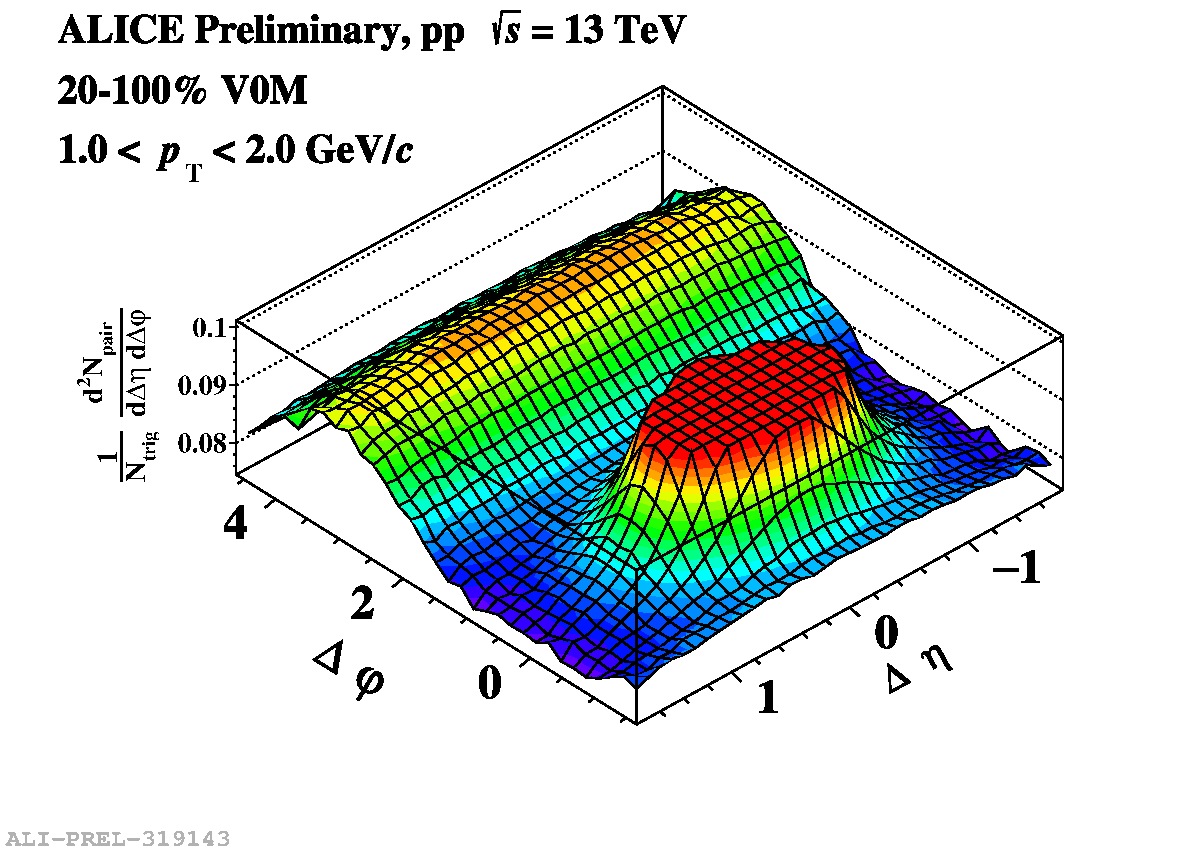
\includegraphics[width=0.31\textwidth]{./figures/corr3.pdf} }
	\caption{ Two-dimensional associated yield per trigger particle as function of $\Delta\eta$ and $\Delta\varphi$ in 0-0.1\% (left), 5-20\% (middle) and 20-100\% (right) multiplicity class. The interval of transverse momentum of trigger particle and associated particle is 1.0$<\it{p}_{\rm{T}}<$2.0 GeV/\it{c}\rm{}. }

\end{figure}

The one-dimensional $\Delta\varphi$ distribution is shown in Figure 2 for pairs of particles with various $\it{p}_{\rm{T}}$ intervals in very high multiplicity class. The associated yield per trigger particle is compared with CMS results. The near-side peak is highest in the 1.0$<\it{p}_{\rm{T}}<$2.0 interval and gradually decreases with increasing $\it{p}_{\rm{T}}$.

The spectra of the ridge yield is shown in Figure 3 in very high multiplicity class and compared with CMS results. The estimator of particle multiplicity of ALICE is done with forward subsystem(V0), whereas that of CMS is done by mid-rapidity particles meeting with the condition of $|\eta|<$2.4 and $\it{p}_{\rm{T}}>$0.4 GeV/\it{c}\rm{}. Dedicated comparison is conducted and the difference of particle multiplicity is estimated to be about 20\%. Taking into account the difference in acceptance of charged tracks and comparable definition of multiplicity,, the measurements are can be considered comparable with each other.


\begin{figure}
	\centering
	\subfigure{ 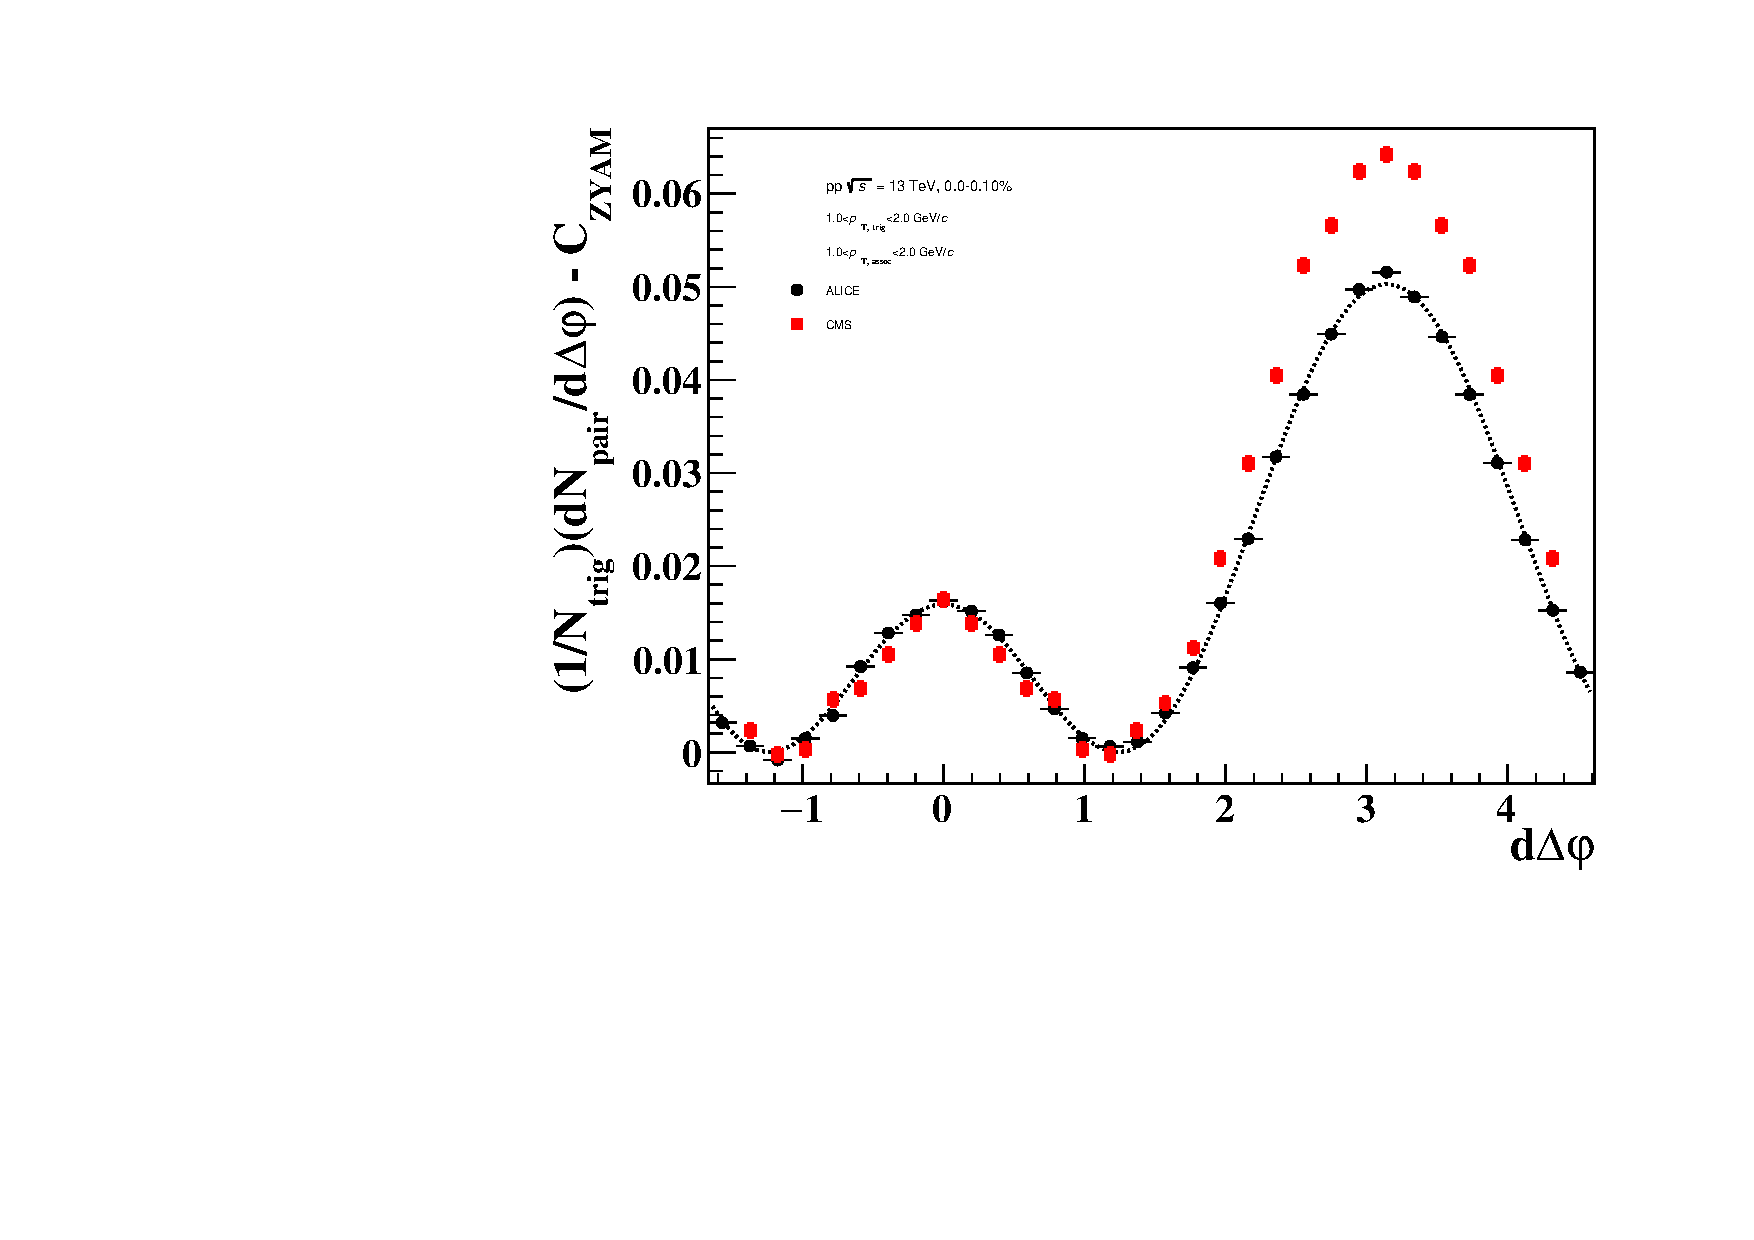
\includegraphics[width=0.31\textwidth]{./figures/dp1.pdf} }
	\subfigure{ 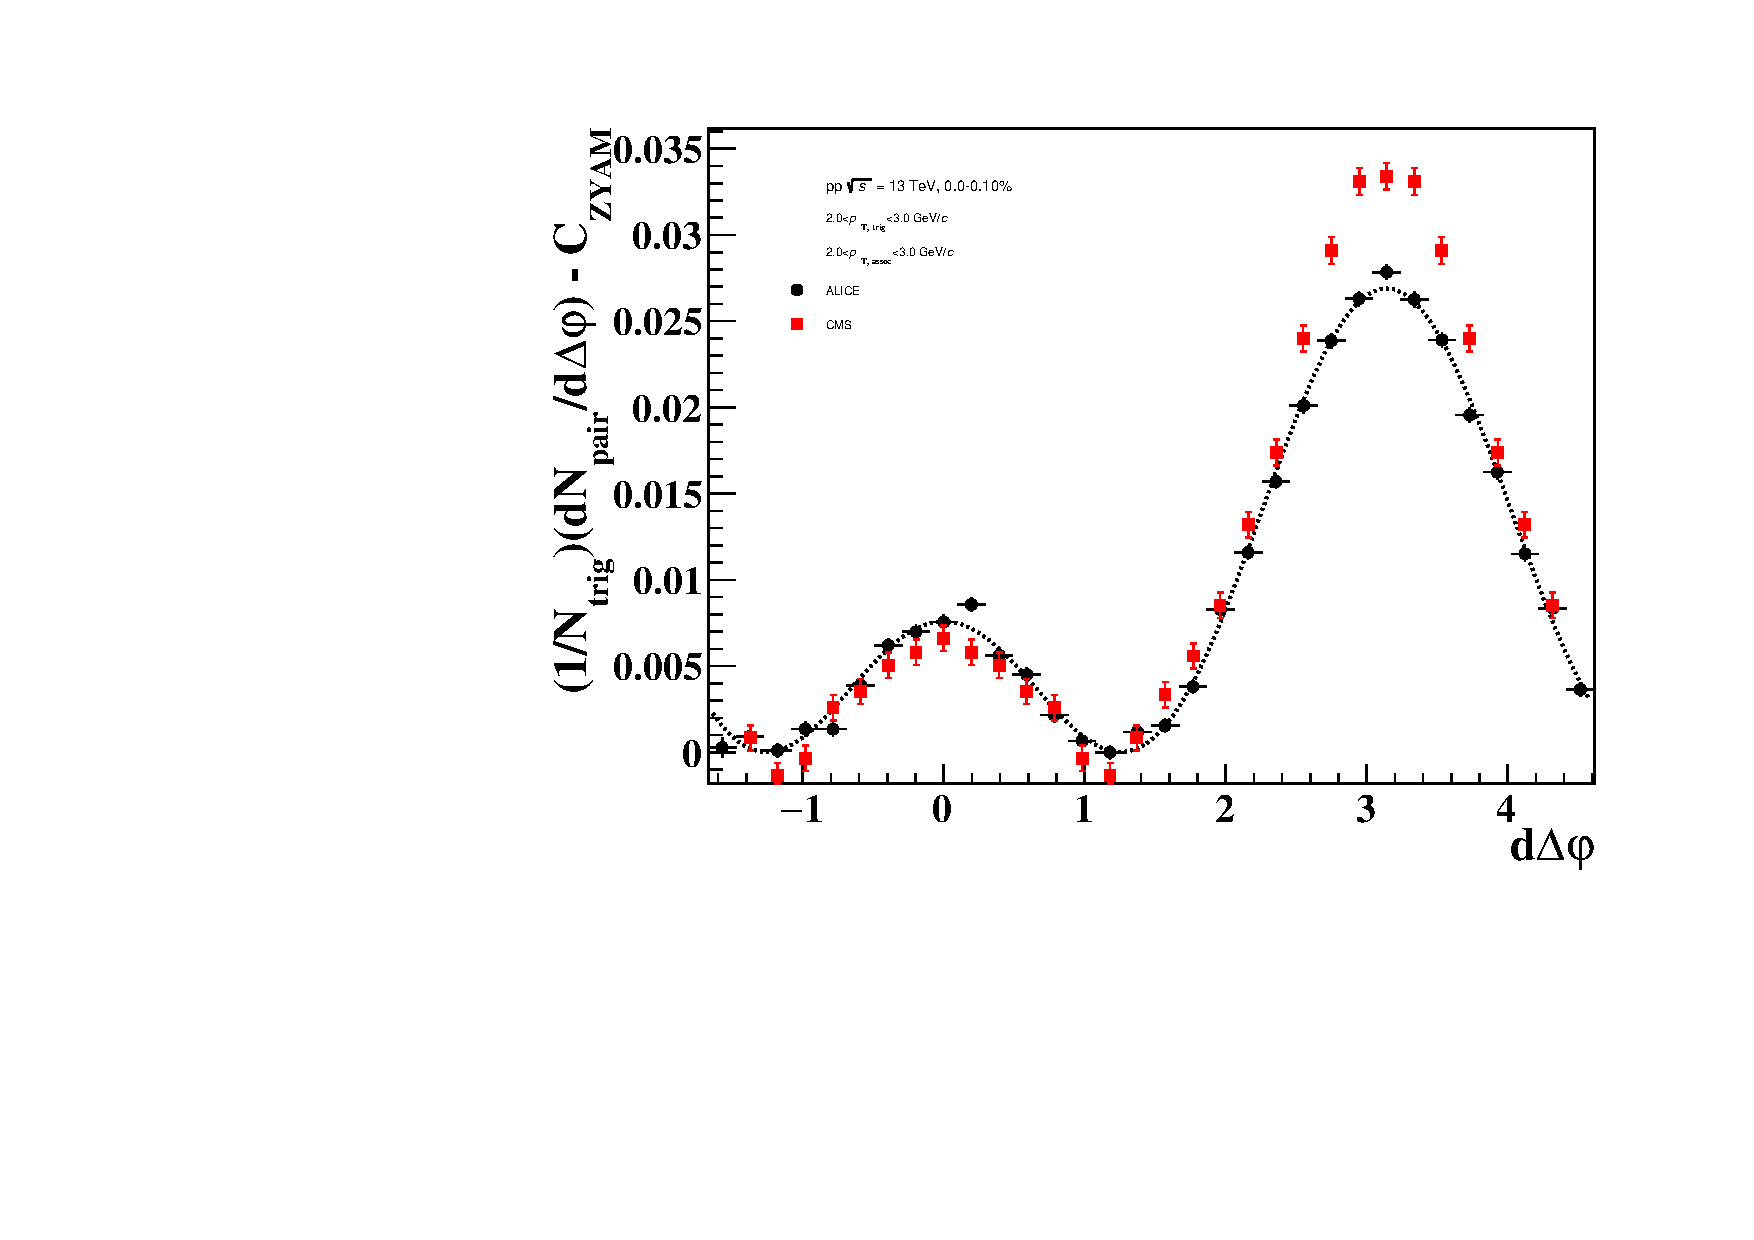
\includegraphics[width=0.31\textwidth]{./figures/dp2.pdf} }
	\subfigure{ 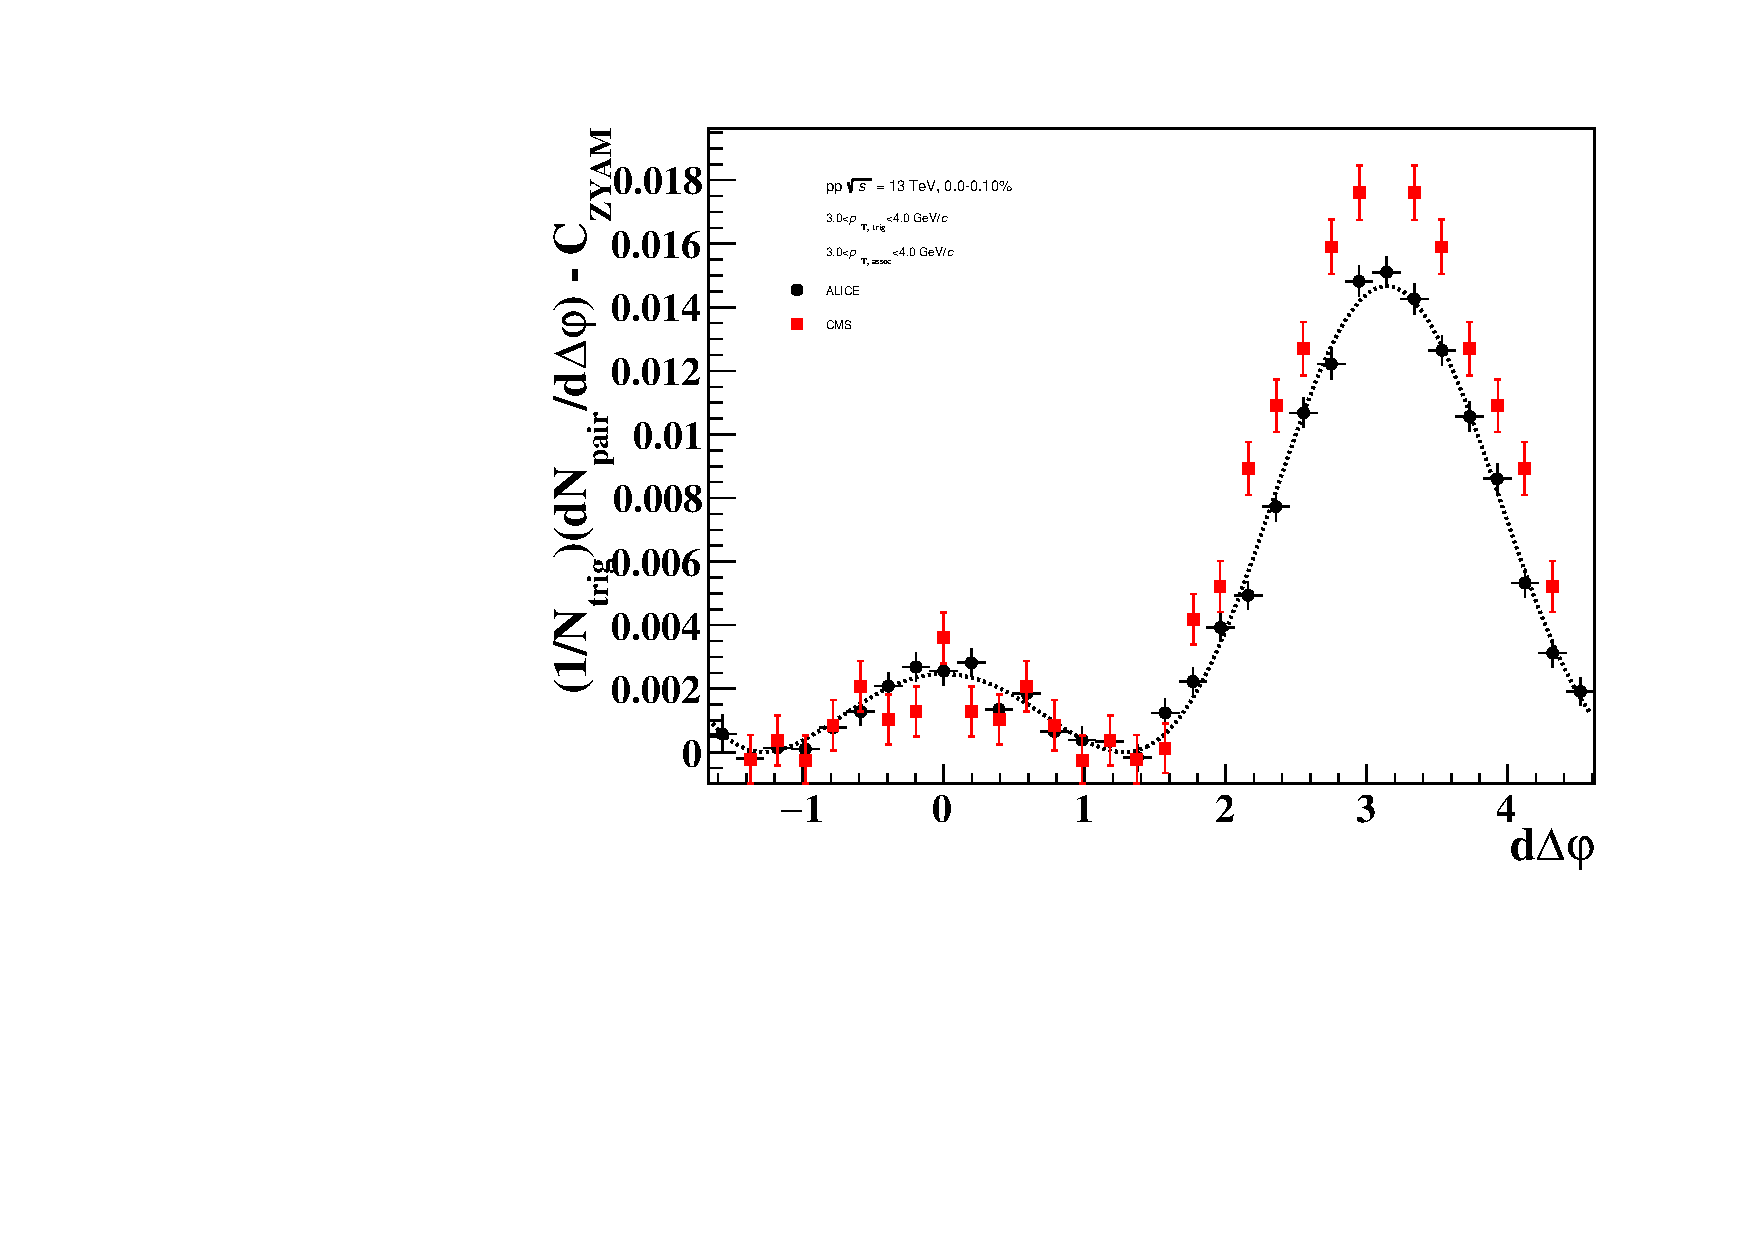
\includegraphics[width=0.31\textwidth]{./figures/dp3.pdf} }
	\caption{ One-dimensional $\Delta\varphi$ distribution in the large $\Delta\eta$ with various transverse momentum intervals. Interval of transverse momentum of trigger particle and associated particle is 1.0$<\it{p}_{\rm{T}}<$2.0 GeV/\it{c}\rm{} (left), 2.0$<\it{p}_{\rm{T}}<$3.0 GeV/\it{c}\rm{} (middle) and 3.0$<\it{p}_{\rm{T}}<$4.0 GeV/\it{c}\rm{} (right), respectively. }

\end{figure}
 
\begin{figure}
	\centering
	\subfigure{ 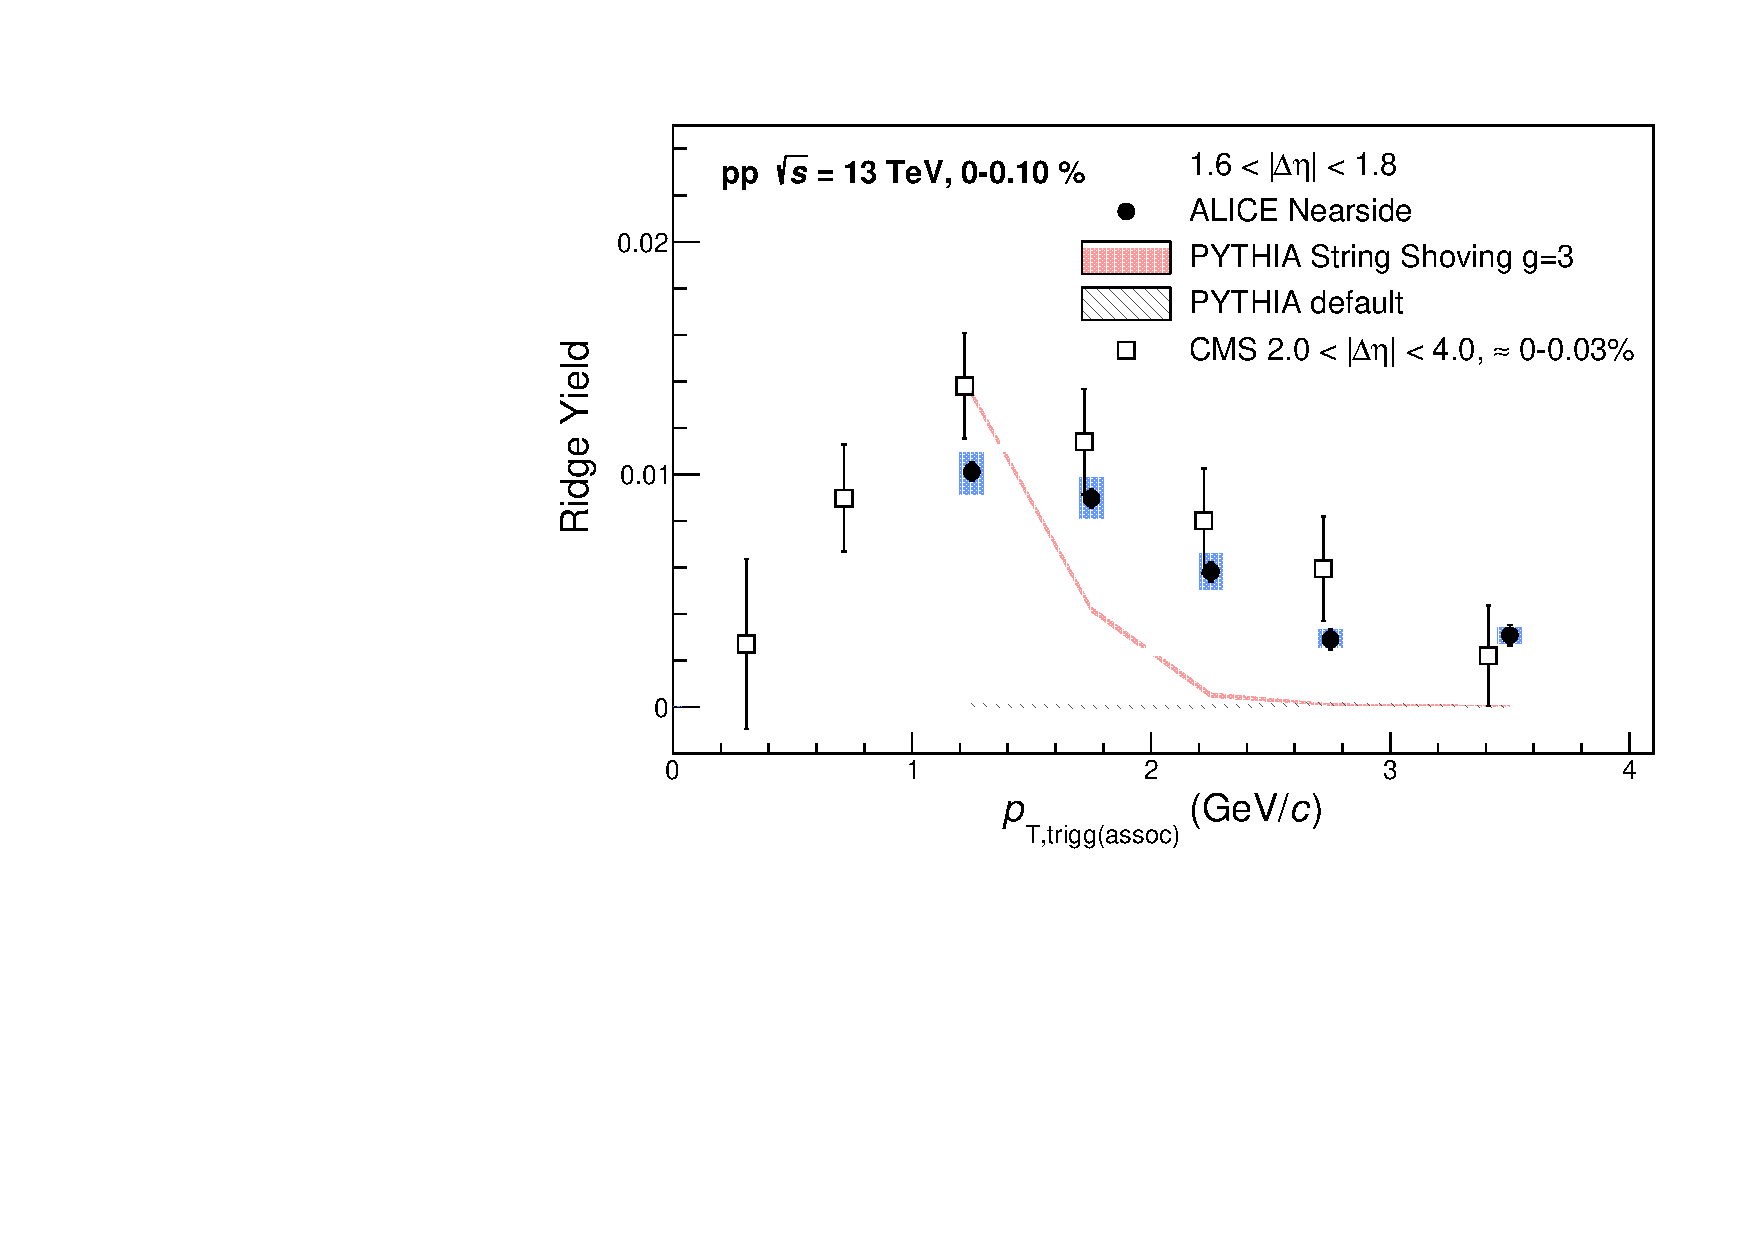
\includegraphics[width=0.7\textwidth]{./figures/Fig1_RidgeYield.pdf} }
	\caption{(color online) The spectra of ridge yield as function of transverse momentum. The spectrum is compared with CMS result \cite{ridge_pp_1}.}
\end{figure}


\begin{figure}
	\centering
	\subfigure{ 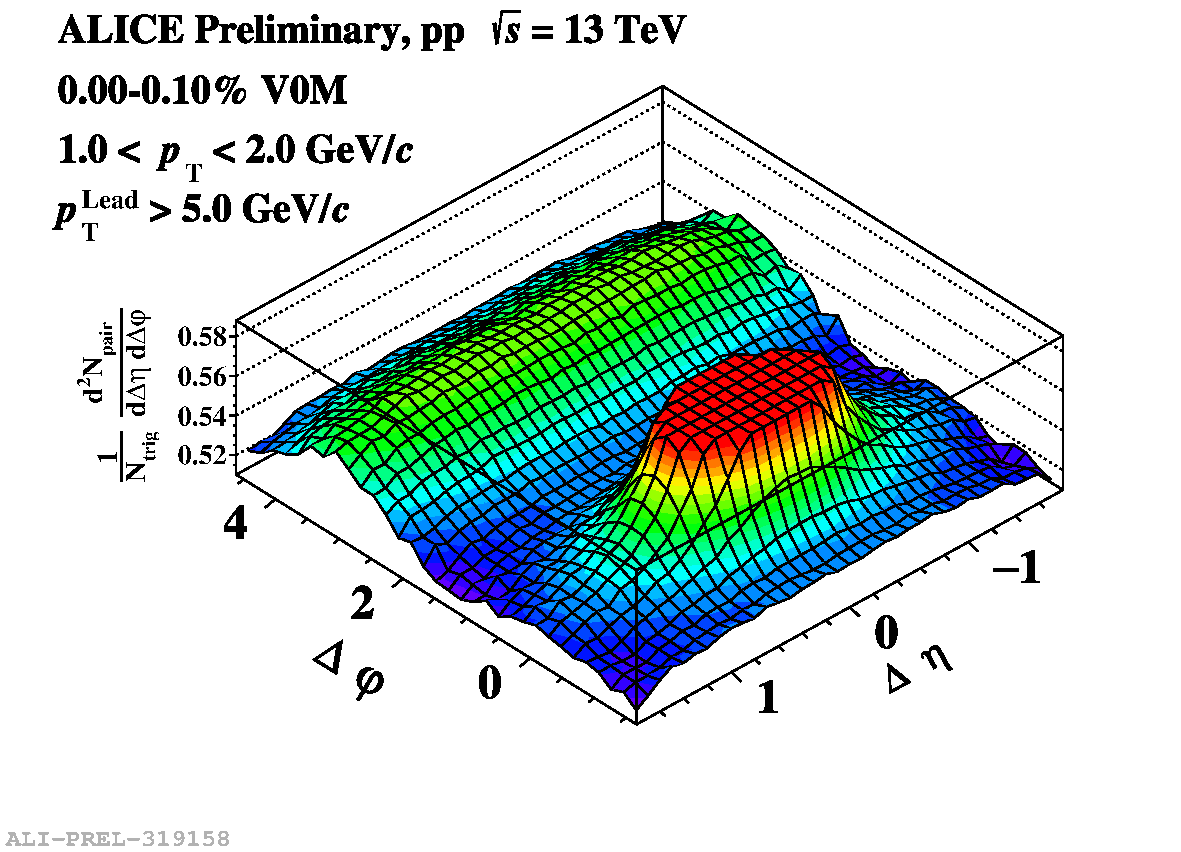
\includegraphics[width=0.4\textwidth]{./figures/corrl1.pdf} }
	\subfigure{ 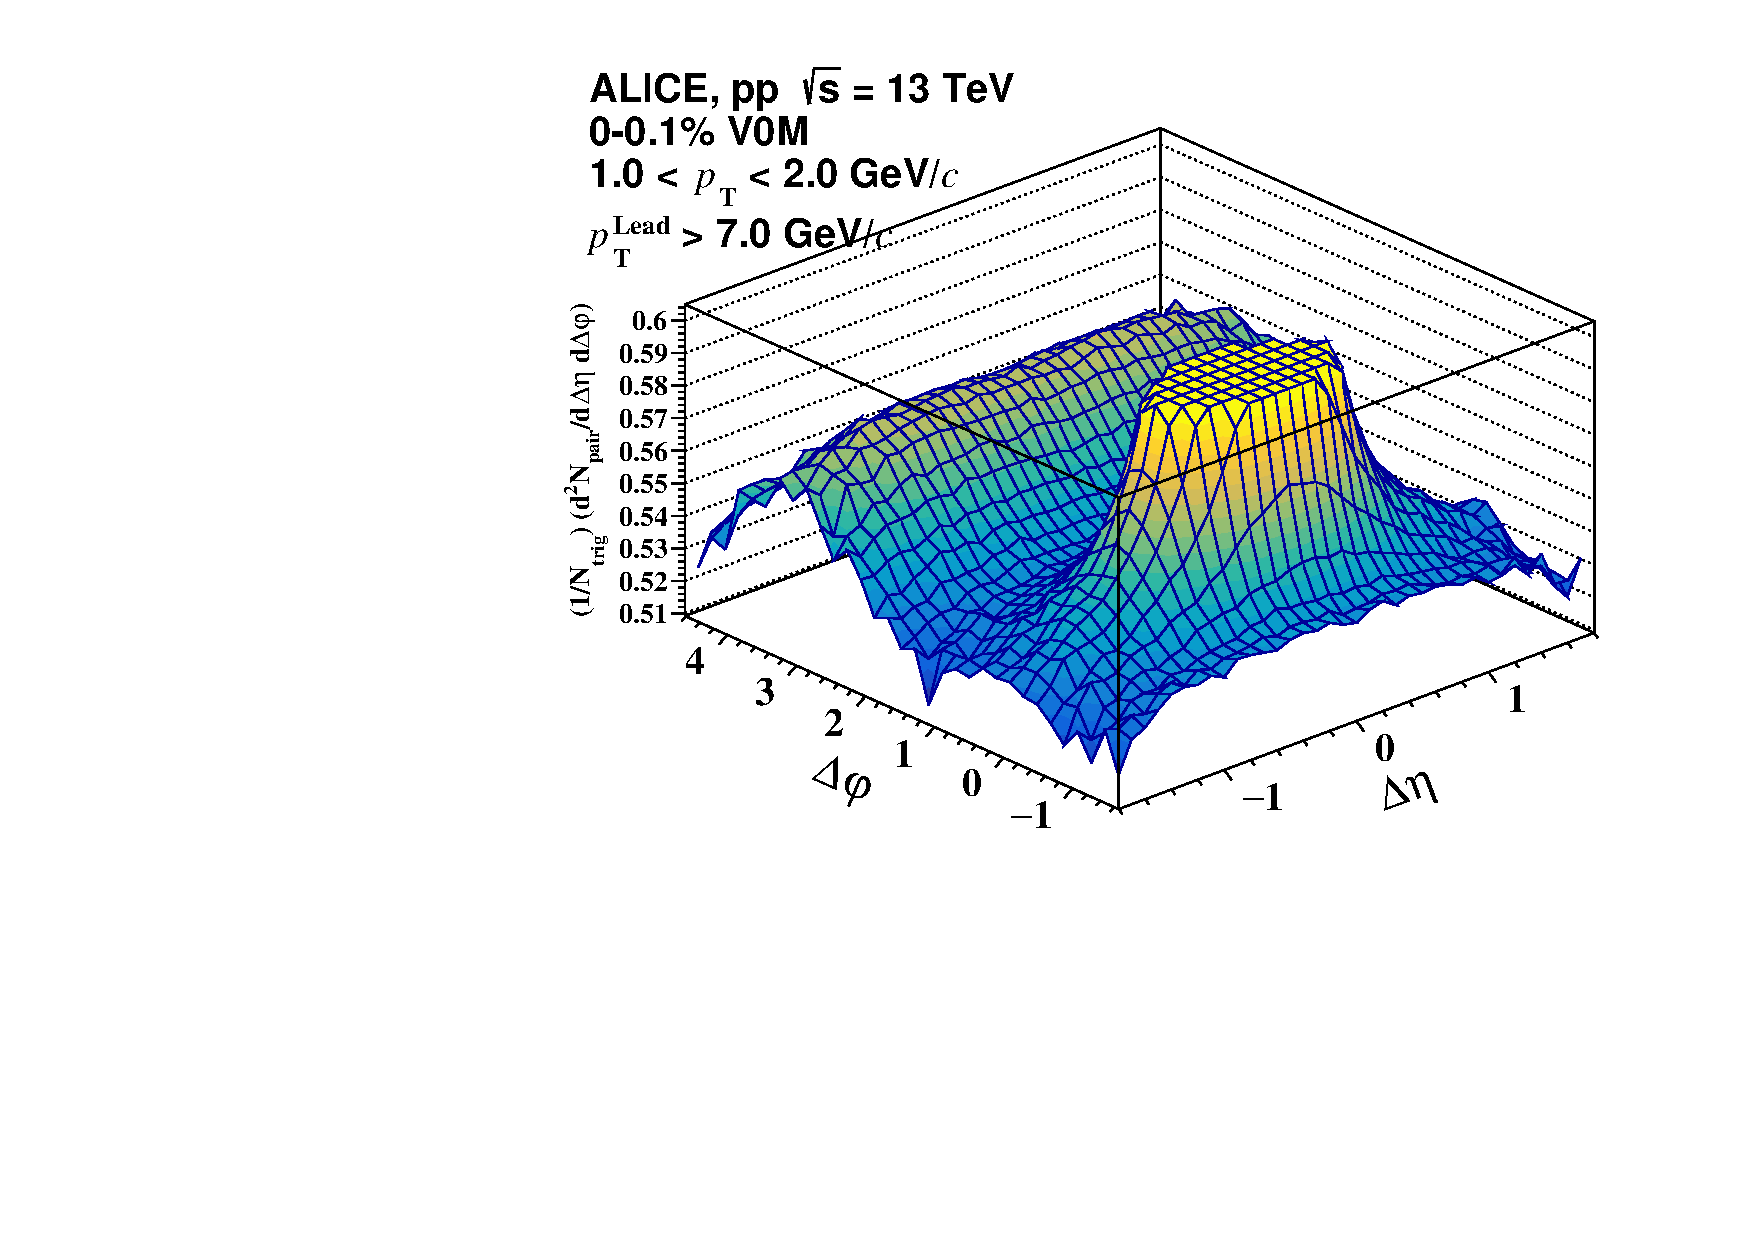
\includegraphics[width=0.4\textwidth]{./figures/corrl2.pdf} }
	\caption{ Two-dimensional associated yield per trigger particle as function of $\Delta\eta$ and $\Delta\varphi$ in top 0-0.1\% multiplicity class. The interval of transverse momentum of trigger particle and associated particle is 1.0$<\it{p}_{\rm{T}}<$2.0 GeV/\it{c}\rm{} for the plots. Threshold for leading track selection is 5 GeV/\it{c}\rm{} (left) and 7 GeV/\it{c}\rm{} (right), respectively. }
\end{figure}


\begin{figure}
	\centering
	\subfigure{ 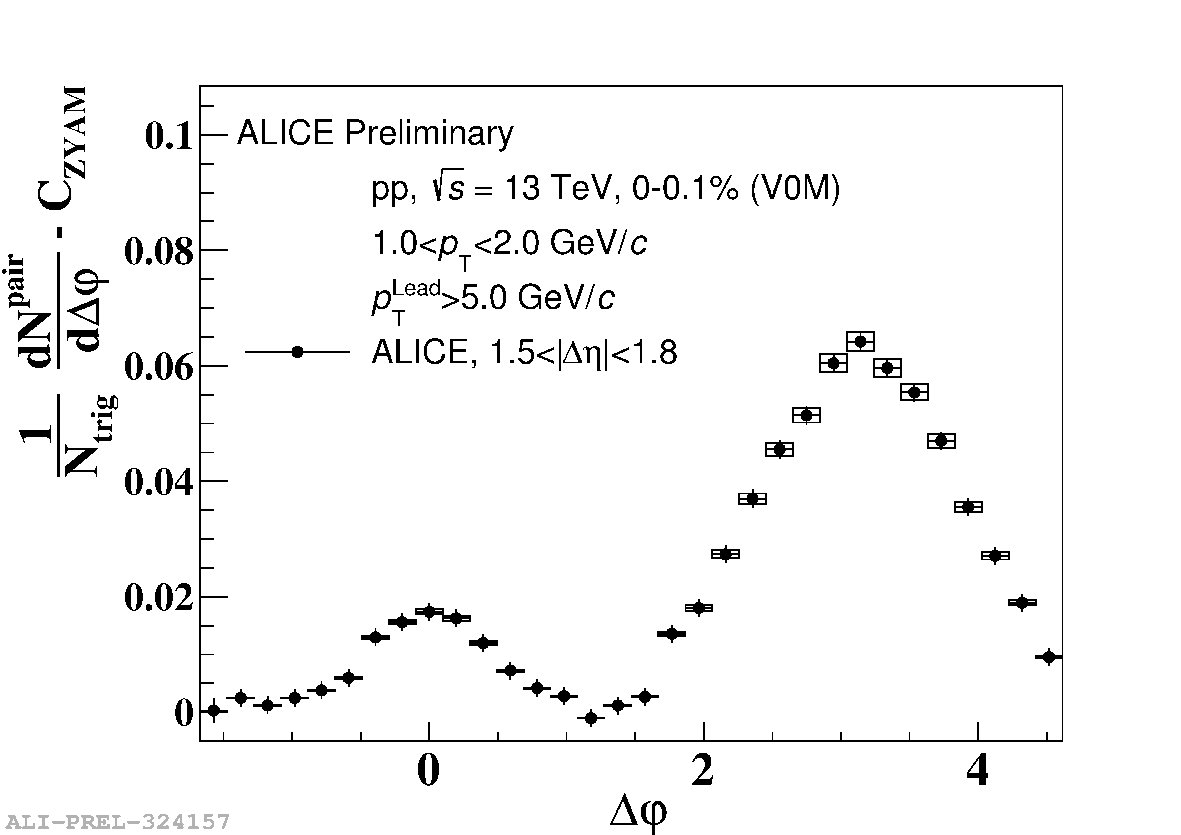
\includegraphics[width=0.4\textwidth]{./figures/dpy1.pdf} }
	\subfigure{ 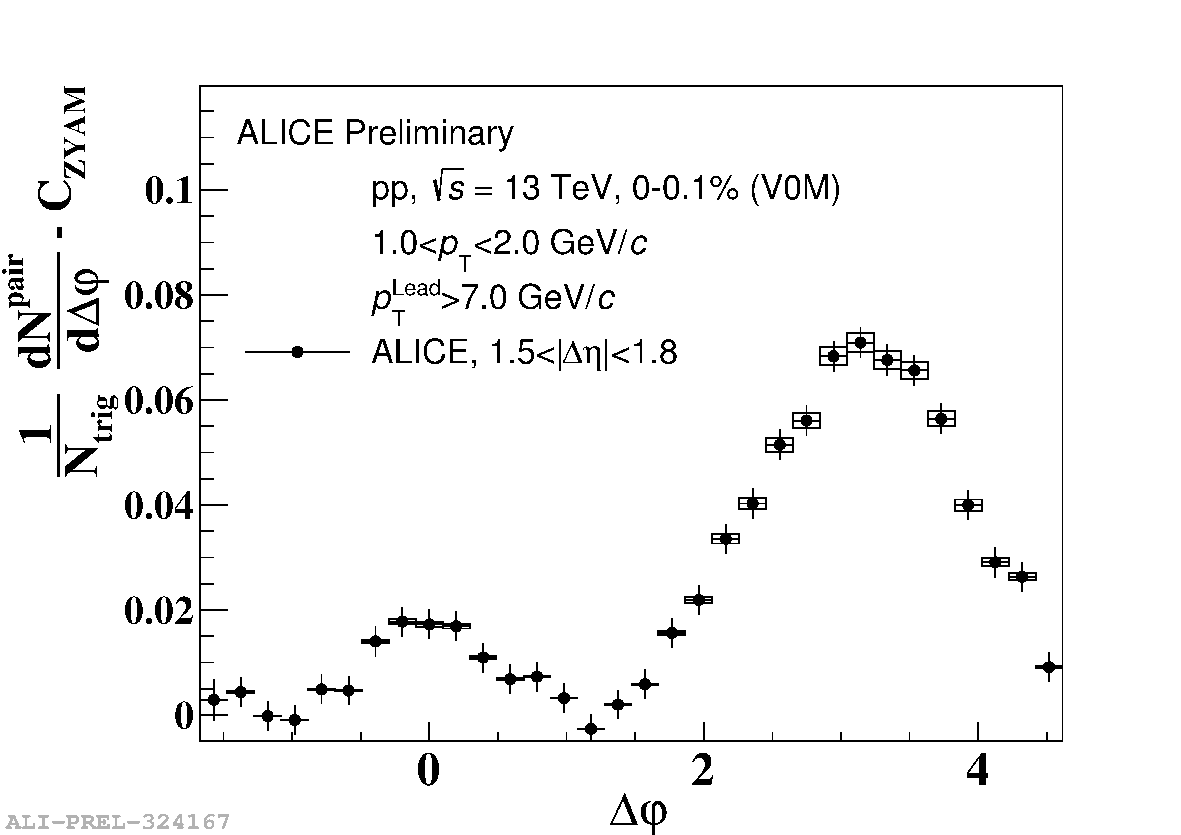
\includegraphics[width=0.4\textwidth]{./figures/dpy2.pdf} }
	\caption{ One-dimensional $\Delta\varphi$ distribution in the large $\Delta\eta$ with various leading track selection thresholds. Interval of transverse momentum of trigger particle and associated particle is 1.0$<\it{p}_{\rm{T}}<$2.0 GeV/\it{c}\rm{}. Threshold for leading track selection is 5 GeV/\it{c}\rm{} (left) and 7 GeV/\it{c}\rm{} (right) respectively. }
\end{figure}


\begin{figure}
	\centering
	\subfigure{ 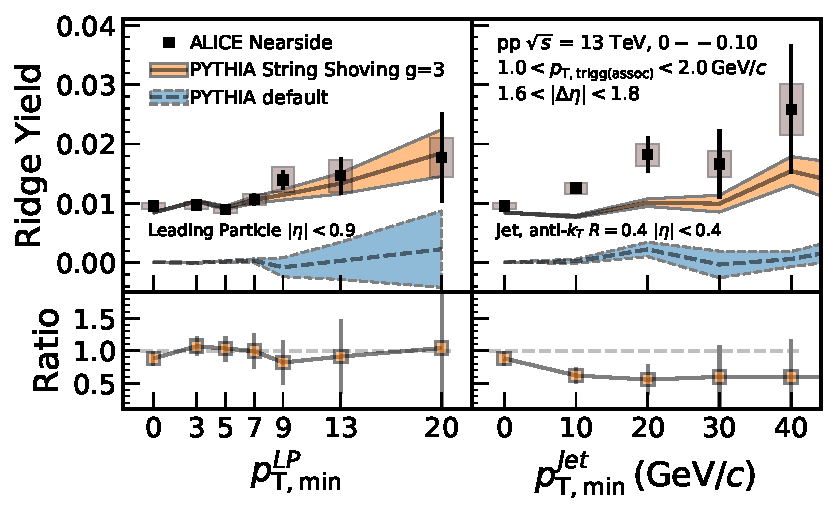
\includegraphics[width=0.8\textwidth]{./figures/Fig2_RidgeYield_Esel_py.pdf}}
	\caption{ The ridge yield spectrum with respect to the leading particle and jet selections. The ridge yields are identical within uncertainties.}
\end{figure}

To further understand the behavior of the ridge in events including hard processes, the two-dimensional associated yield per trigger particle is measured with the leading track selection as shown in Figure 4. The ridge is still visible in the events where $\it{p}_{\rm{T}}^{\rm{Lead}}>$7 GeV/c, which means that the ridge co-exists with hard-scattering in pp collisions. 

The one-dimensional $\Delta\varphi$ distribution with the leading track selection is shown in Figure 5. The near-side yield doesn't change with respect to the leading track requirements within the uncertainties, whereas the away-side peak increases as the leading track requirement gets stronger, presumably because of the increase of the recoil jet yield.

The ridge yield is inspected as a function of the leading track selection in Figure 6. As seen in the previous plots, the ridge yield does not depend on the selection, which indicates that the ridge is not affected significantly by the hardness of the events.

\section{Model Comparison}
\label{sec:theory}



% !TEX root = paper.tex

\section{Conclusions}
\label{sec:summary}

Long- and short-range correlations for pairs of charged particles with 1~$ < \pt < $~4~GeV/$c$ are studied in pp collisions at $\sqrt{s} = 13$~TeV with a focus on high-multiplicity events. The ridge and near-side jet yields are extracted and their event scale dependence have been studied. The obtained long-range ridge yields are compatible to those observed by the CMS collaboration~\cite{Khachatryan:2015lva}.
%In addition, the $\pt$ and the $\it{p}_{\rm{T,Lead}}$ or $\it{p}_{\rm{T,Jet}}$ selection dependence of the long-range azimuthal correlations are measured.
The $\pythiashoving$ model describes the observed yields qualitatively but the yields it predicts decrease more rapidly with increasing $\pttrigassoc$ than those measured. On the other hand, the $\epos$ model gives a better description for the $\pttrigassoc$ dependence while overestimating the ridge yield for $\pttrigassoc<$~2 GeV/$c$. Finally, no long-range ridge is formed in The $\pythiam$ model.
%Furthermore the ridge yields are studied in events, where jets with a harder fragmentation are preferred by requiring the minimum value of the transverse momentum of leading particles in each event $\ptlead$ or the one of reconstructed jets $\ptjet$. The ridge structure still persist with both selections. The ridge yields increase as $\ptlead$ and $\ptjet$ increase. The latter, however, is more significant than the former selection. The results are compared with $\pythiashoving$ calculations, showing the enhancement while underestimating the absolute ridge yield.

The ridge yields are further studied in high-multiplicity events biased with additional event-scale selections, which impose a minimum transverse momentum cutoff on a leading track or jet. The ridge structure still persists with both selection criteria. The ridge yields increases as $\ptlead$ and $\ptjet$ increase. $\pythiashoving$ and $\epos$ estimate qualitatively the trends for the event-scale selections. However, the former underestimates and the latter overestimates it. The model predictions are also compared with the yield of the near-side jet-like correlation measured in the biased events. The evolution of the near-side jet yield as a function of event-scale $\pt$ is better captured by $\epos$, while the $\pythiashoving$ calculation tends to overshoot the data. 
%which results in opposite trends between the ridge yield and near-side jet-like correlations.
The results might open a new way of studying the impact parameter dependence of small systems with jet tagged events in the future and will help to constrain the physical origins of long-range correlations.


%%%%% acknowledgements
\newenvironment{acknowledgement}{\relax}{\relax}
%\begin{acknowledgement}
%\section*{Acknowledgements}
%\input{acknowledgements.tex}    %%%%%%% done by webmaster team
%\end{acknowledgement}

%%%%%%%% Bibliography (In case of using bibtex generate the bbl requested by arXiv)
%\bibliographystyle{utphys}   % Remember we use title in the biblio
%\bibliography{biblio}
%\input {bibliography.tex}

%%%%%%%%% appendix with author list
\newpage
\appendix
%
%\input{}               %%%%%%%%%%% put your appendices here
%





%\section{The ALICE Collaboration}
%\label{app:collab}
%\input{authorlist-preprint.tex}  %%%%%%% done by webmaster team


\clearpage

\bibliographystyle{utphys}
\bibliography{paper.bib}

%%%%%%%%% appendix with author list
%\section{The ALICE Collaboration}
%\label{app:collab}
%\input{Alice_Authorlist_2017-Aug-21.tex}  %%%%%%% done by webmaster team
%\input{}     


\end{document}
